\documentclass{article}
\usepackage{graphicx}
\usepackage{hyperref}

\usepackage{enumitem}

\begin{document}

\title{Monte Carlo, Exercise Session 3}
\author{Alexey Sofiev, 013573003}

\maketitle

%\begin{abstract}
%The abstract text goes here.
%\end{abstract}

\section{Exercise 1}
Files: Ex1.*. 

\textbf{Answer:} Figure \ref{fig:ex1_answer}.

\begin{figure}[!hbt]
	\centering
	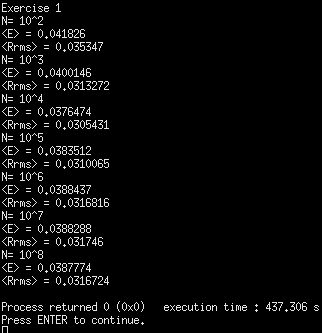
\includegraphics[width=4.3in]{ex1_answer}
	\caption{Ex1 answer.}
	\label{fig:ex1_answer}
\end{figure}

The other main question is log- plot, visualized in Figure \ref{fig:ex1_log}.

\begin{figure}[!hbt]
	\centering
	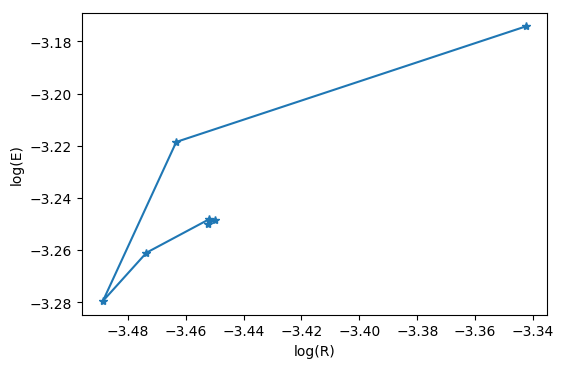
\includegraphics[width=4.3in]{ex1_log}
	\caption{Ex1 log plot.}
	\label{fig:ex1_log}
\end{figure}

And point in the upper right corner is obtained at the smallest N=100. (line connects to N=$10^3 \rightarrow 10^4 ...$) Therefore, the maximal absolute value of log(E) allowed should be 3.29.
\\
\\
\textbf{Solution details:}

%\begin{enumerate}[noitemsep]
	\textbf{1.} Algorithm is done basing on page 8 from \href{$https://moodle.helsinki.fi/pluginfile.php/714567/mod_resource/content/8/Markov_chain.pdf$}{Lecture notes on MCMC.}
%\end{enumerate}

	\textbf{2.} V is set to 1.
	
	\textbf{3.} Setting the range and $\triangle X_{max}$	

First let's take a look at the function without zooming. Figure \ref{fig:ex1_fig05}
\begin{figure}[!hbt]
	\centering
	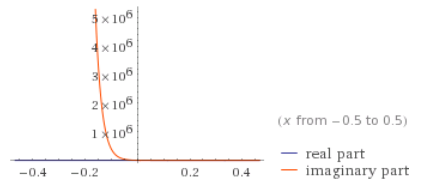
\includegraphics[width=4.3in]{ex1_fig05}
	\caption{Ex1, view on the function with 0.5. Function plotted with wolframalpha.}
	\label{fig:ex1_fig05}
\end{figure}

It can be noticed, that it is pretty flat, so now lets zoom into interesting part, Figure \ref{fig:ex1_fig008}.

\begin{figure}[!hbt]
	\centering
	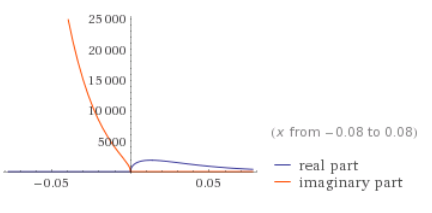
\includegraphics[width=4.3in]{ex1_fig008}
	\caption{Ex1, autozoom into real part. Function plotted with wolframalpha.}
	\label{fig:ex1_fig008}
\end{figure}

From Figure \ref{fig:ex1_fig008} it can be seen that setting $x_0$ to vary from 0 to 0.1, and $\triangle X_{max}$ to 0.05 is enough to generate most values. From lecture notes, it is told that $x_0$ doesn't really matter, on a long run, all the generated values will be distribution based distributed.

After generating random values and plotting them, the distribution obtained is presented in Figure \ref{fig:ex1_myDistribution}.

\begin{figure}[!hbt]
	\centering
	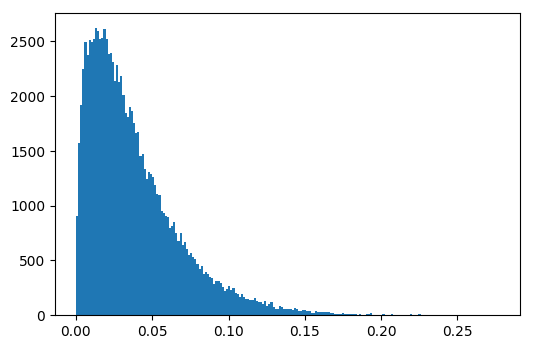
\includegraphics[width=4.3in]{ex1_myDistribution}
	\caption{Ex1, histogram of random values provided by the code.}
	\label{fig:ex1_myDistribution}
\end{figure}

The shape looks pretty much according to the theory presented in earlier figures.


\clearpage

\section{Exercise 2}
This exercise requires a lot of plotting, so will be done in Python using the Mersenne twister. File: Ex2.py

\textbf{Synthetic data:}

Using the lecture notes, the synthetic data, two of which are visualized in Figures \ref{fig:ex2_synt1} and \ref{fig:ex2_synt2}, is generated.
\begin{figure}[!hbt]
	\centering
	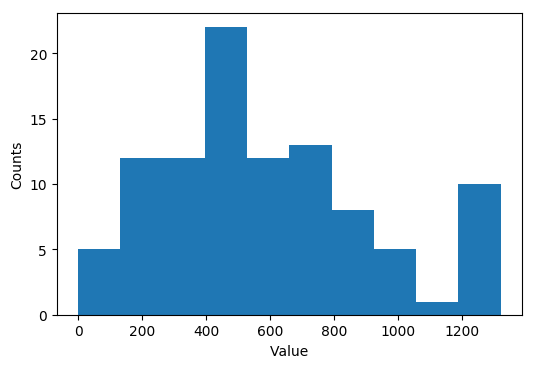
\includegraphics[width=4.3in]{ex2_synt1}
	\caption{Ex2, an example of generated synthetic data.}
	\label{fig:ex2_synt1}
\end{figure}

\begin{figure}[!hbt]
	\centering
	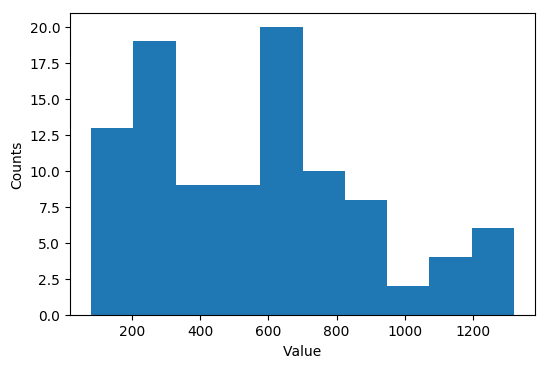
\includegraphics[width=4.3in]{ex2_synt2}
	\caption{Ex2, an example of generated synthetic data.}
	\label{fig:ex2_synt2}
\end{figure}

The generated synthetic data of 100, is has some sort of similarity, but they are still different.



\end{document}